\documentclass[letterpaper,11pt]{article}
\usepackage{myCV}

% bibliography
\usepackage{natbib}
\usepackage{bibentry}

% meta data
\name{A Cool Cat}
\email{coolcat@mail.com}
\profile{profile.jpg}
\setProfileWidth{3.5cm}

\addlink
    {https://scholar.google.com/citations?user=N2-7ArsAAAAJ&hl=en}
    {Google Scholar 
\includegraphics[height=0.3cm]{icon/google-scholar.png}}
\addlink
    {https://orcid.org/0000-0001-7843-1925}
    {ORCID 
\includegraphics[height=0.3cm]{icon/orcid.png}}
\addlink
    {https://github.com/liu-qilong}
    {GitHub 
\includegraphics[height=0.3cm]{icon/github.png}}
\addlink
    {https://qilong-liu.vercel.app}
    {Homepage 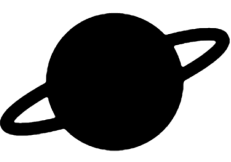
\includegraphics[height=0.3cm]{icon/blog.png}}

\addinfo{Position}{Cat}
\addinfo{Base}{Hong Kong}
\addinfo{Salary Expectation}{HKD 200w}
\addinfo{Institution}{CoolCat Ltd.}

\begin{document}
    \maketitle

    % research interests
    \section{Research interests}

    \begin{resumeItemize}
        \item 3D computer vision; 4D scene reconstruction; Dense motion tracking; Statistical human modeling; Human-computer interaction; AI for design.
    \end{resumeItemize}
    
    % education
    \section{Education}

    \resumeColumnsStart
        \resumeEntry
            {The Hong Kong Polytechnic University
            }{Sep 2021 -- Feb 2024}
            {Master of Philosophy}{Hong Kong, China}
        \resumeSubline
            {and AiDLab}{}
        \resumeSubline
            {Supervised by Prof. Kit-lun Yick and co-supervised by Prof. Joanne Yip and Dr. Yue Sun}
    \resumeColumnsEnd

    % awards
    \section{Awards}

    \resumeColumnsStart
        \resumeEntry
            {The Hong Kong Polytechnic University Research Studentship}{2021 -- 2023}
            {The Hong Kong Polytechnic University}{}
    \resumeColumnsEnd

    % publications
    \section{Publications}

    \bibliographystyle{unsrt}
    \nobibliography{publications.bib}

    \begin{resumeItemize}
        % \item \textbf{In Submission}
        % \item \bibentry{QinfengXiao2024}
        
        % \item \textbf{Under Review}
        
        \item \textbf{Journal}
        \item \bibentry{LiuQilong2024} \paralink{https://jcr.clarivate.com/jcr-jp/journal-profile?journal=PLOS\%20ONE&year=2023}{JCR Q1, IF 2.9}
        \item \bibentry{ZhangLiying2024} \paralink{https://jcr.clarivate.com/jcr-jp/journal-profile?journal=IEEE\%20ACCESS&year=2023}{JCR Q2, IF 3.4}
     \end{resumeItemize}

    % work experience
    \section{Work \& research experience}

    \resumeColumnsStart
        \resumeEntry
            {Shenzhen Base of The Hong Kong Polytechnic University}{Dec 2020 -- Jun 2021}
            {Student Assistant (part-time) for \href{https://research.polyu.edu.hk/en/persons/kit-lun-yick}{Prof. Kit-lun Yick}}{Shenzhen, Guangdong, China}
            \resumeSubline{Supervised by \href{https://research.polyu.edu.hk/en/persons/kit-lun-yick}{Prof. Kit-lun Yick}}
            \resumeSubline{3D/4D scanning data cleansing, labelling, and processing}
        \resumeEntry
            {Shenzhen Zhishixinyun Educational Technology Ltd.}{Nov 2019 -- Mar 2020}
            {Cofounder and Python tutorial lecturer}{Shenzhen, Guangdong, China}
            \resumeSubline{A campus startup that aims at providing short-term STEM and arts tutorials for college students}
    \resumeColumnsEnd

    % skills
    \section{Skill set}

    \begin{resumeItemize}
        \item \textbf{Languages}. English (fluent); Mandarin (native); Cantonese (native)
        \item \textbf{Programming}. PyTorch \& Python (seasoned); JavaScript \& Node.js \& CSS \& HTML (seasoned); Bash shell scripting (intermediate); C/C++ (basic); Matlab (intermediate)
        \item \textbf{Others}. LaTeX (seasoned); TikZ (intermediate); I am also a self-estimated good cook.
    \end{resumeItemize}

\end{document}
